\documentclass[12pt, letterpaper, twoside]{article}
\usepackage[sectionbib,round]{natbib}
\bibliographystyle{apalike}
\usepackage[utf8]{inputenc}
\usepackage{amsmath}
\usepackage{graphicx} %Loading the package
\graphicspath{{../plots/}} %Setting the graphicspath
\usepackage{aas_macros} %commom journal
\usepackage{physunits}
\usepackage{times}
\usepackage{import}

\begin{document}

\section{Signal-to-noise ratio}

The signal-to-noise ratio (SNR or just SN) is a measure used in signal analysis. The measurement of a signal is always accompanied by some noise, whether it is intrinsic to the measuring device, from external sources that cannot be disentegled from the object of interest or from the medium between the source and the measuring device. The SNR can provide a measure of the intensity of the desired signal against the background signal. A commom definition of SNR is
\begin{equation}
	\label{eq:snr_commom_def}
	\text{SNR} = \frac{P_{\text{signal}}}{P_{\text{noise}}} \, ,
\end{equation}
where $P_{\text{signal}}$ and $P_{\text{noise}}$ are respectivelly the average power of signal and noise. By this definition one can conclude that SNR is a dimensionless quantity.

Altought in images processing, another definition is commonly used: 
\begin{equation}
	\label{eq:snr_image_def}
	\text{SNR} = \frac{S}{\sigma} \, ,
\end{equation}
where $S$ is the average of the desired signal and $\sigma$ is average of its uncertainty. In particular, for spectroscopy, the $S$ is the spectral flux density measured for example in \erg/\s/\cm$^{2}$/\AA. For a variable continous signal $S(\lambda)$ which depends on the wavelength $\lambda$ and a variance $\sigma^{2}(\lambda)$ as uncertanty, one can measure obtain the average in an interval $\Delta\lambda$ of both signal by \citep{cappellari+03}:
\begin{equation}
	\label{eq:avg_cont_signal}
	S = \dfrac{1}{\Delta\lambda}\int_{\Delta\lambda} S(\lambda)\mathrm{d}\lambda
	\quad \text{and} \quad
	\sigma^{2} = \dfrac{1}{\Delta\lambda}\int_{\Delta\lambda} \sigma^{2}(\lambda)\mathrm{d}\lambda \, .
\end{equation}

However, spectra are most commonly obtained as discrete signals within $n$ wavelength intervals $\delta\lambda_{j}$. Then the equation \ref{eq:avg_cont_signal} becomes:
\begin{equation}
	S = \dfrac{\sum\limits_{j=1}^{n} S(\lambda_{j}) \delta\lambda_{j}}{\sum\limits_{j=1}^{n} \delta\lambda_{j}}
	\quad \text{and} \quad
	\sigma^{2} = \dfrac{\sum\limits_{j=1}^{n} \sigma^{2}(\lambda_{j}) \delta\lambda_{j}}{\sum\limits_{j=1}^{n} \delta\lambda_{j}}
\end{equation}
for $\delta\lambda_{j}$ uniform throughout wavelength range then $\delta\lambda = \delta\lambda_{j}$ for all $j$. Thus
\begin{equation}
	S = \dfrac{\delta\lambda \sum\limits_{j=1}^{n} S(\lambda_{j})}{n\delta\lambda}
	\quad \text{and} \quad
	\sigma^{2} = \dfrac{\delta\lambda \sum\limits_{j=1}^{n} \sigma^{2}(\lambda_{j})}{n\delta\lambda} \, ,
\end{equation}
or yet:
\begin{equation}
	S = \dfrac{1}{n}\sum\limits_{j=1}^{n} S(\lambda_{j})
	\quad \text{and} \quad
	\sigma^{2} = \dfrac{1}{n}\sum\limits_{j=1}^{n} \sigma^{2}(\lambda_{j}) \, .
\end{equation}

Finally the signal-to-noise of a sampled signal is given by
\begin{equation}
	\text{SNR} = \left( \dfrac{1}{\sqrt{n}} \right) \dfrac{\sum\limits_{j=1}^{n} S(\lambda_{j})}{\sqrt{\sum\limits_{j=1}^{n} \sigma^{2}(\lambda_{j})}} \, .
\end{equation}

Thereafter, we apply the previous formulas to obtain a signal-to-noise map of an observation of galaxy NGC 613 made with MUSE spectrograph (Figure \ref{fig:snr_ngc613}).
\begin{figure}[h]
	\label{fig:snr_ngc613}
	\centering
	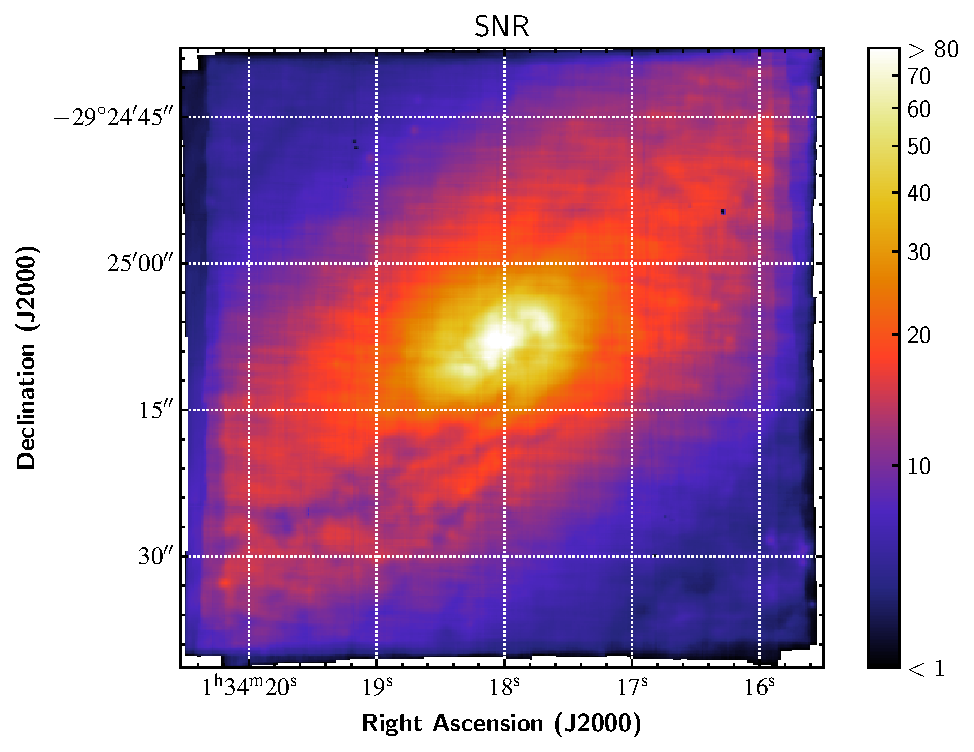
\includegraphics[width = 0.8\linewidth]{snr_muse_ngc613.pdf}
	\caption{Signal-to-noise map of galaxy NGC 613. The observation was done with MUSE spectrograph. The image was enhanced \citep{gonzalez+18} by clipping the intensity range between 1 and 80. The image was colorized was produced by mapping the intensity of each pixel $I(x,y)$ with a color scale using an arcsinh function \citep{lupton+04}.}
\end{figure}

\section{Resampling}

\begin{figure}[h]
	\label{fig:resampling_comparison}
	\centering
	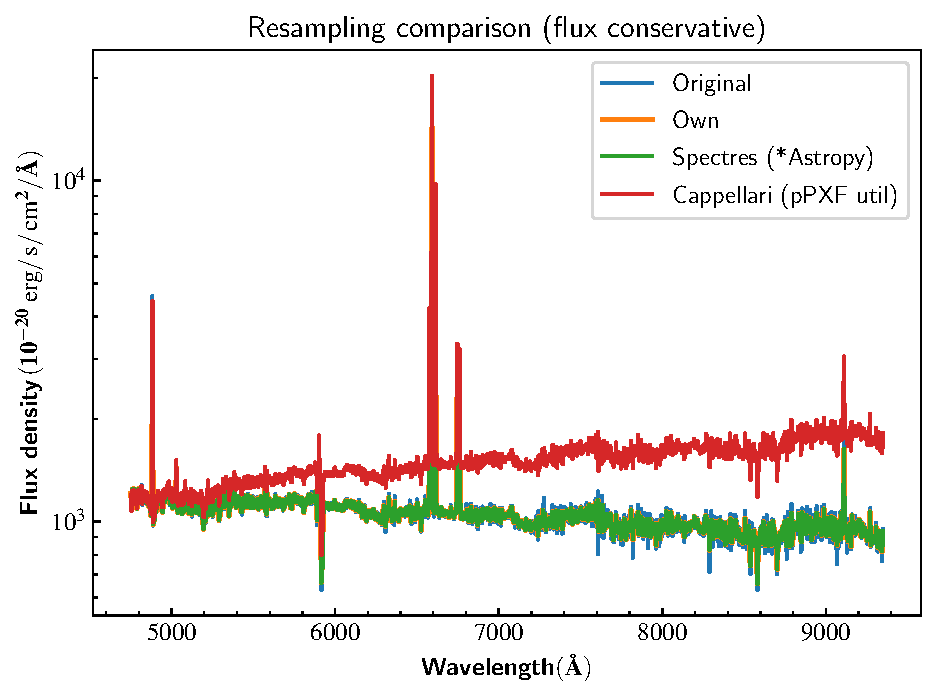
\includegraphics[width = \linewidth]{resampling_comparison.pdf}
	\caption{}
\end{figure}

\begin{table}[h]
	\caption{}
	\label{tab:resampling_comparison}
	\begin{tabular}{lcc}
		\hline
		\import{../tables/}{table_resampling_comparison.tex}
	\end{tabular}
\end{table}

\bibliography{biblio.bib}

\end{document}
